\chapter{\label{ch:6-michel}Study of Michel Electrons in ProtoDUNE--SP} 

\minitoc

This chapter will cover the primary analysis of this thesis; a study of Michel
electrons in the ProtoDUNE--SP detector which aims to investigate the agreement
between data and simulation, and to provide an estimate of the energy scale
uncertainty and energy scale bias for electrons in the 0--60 MeV range. 

The work done for this section is ongoing; preliminary work on this topic was
presented in the report submitted for transfer of status. The rest of the work
for this section is expected to be completed by the end of October 2019.

\noindent The work done as of writing for this chapter is as follows:
\begin{itemize}[noitemsep,nolistsep]
	\item Event selection algorithm developed based on clustering of the Michel
	like hits discussed in the previous chapter.
	\begin{itemize}[noitemsep,nolistsep]
		\item Purity of > 98\% and efficiency of 5\% measured in ProtoDUNE--SP 
		simulations.
	\end{itemize}
	\item Two possible energy reconstruction algorithms developed.
	\begin{itemize}[noitemsep,nolistsep]
		\item Cone algorithm.
		\item Semantic segmentation algorithm with U-ResNet CNN architecture.
	\end{itemize}
\end{itemize}

\noindent The work left to do is as follows:
\begin{itemize}[noitemsep, nolistsep]
	\item Validation of algorithms on the real ProtoDUNE--SP data.
	\item Data MC comparison for Michel electron energy spectrum.
	\item Energy scale uncertainty and energy scale bias measurements with 
	measured Michel electron energy spectrum.
\end{itemize}

\noindent An example Michel electron candidate event from the real ProtoDUNE--SP 
data is given in figure \ref{fig:michel_event}.

\begin{figure}[h]
	\centering
	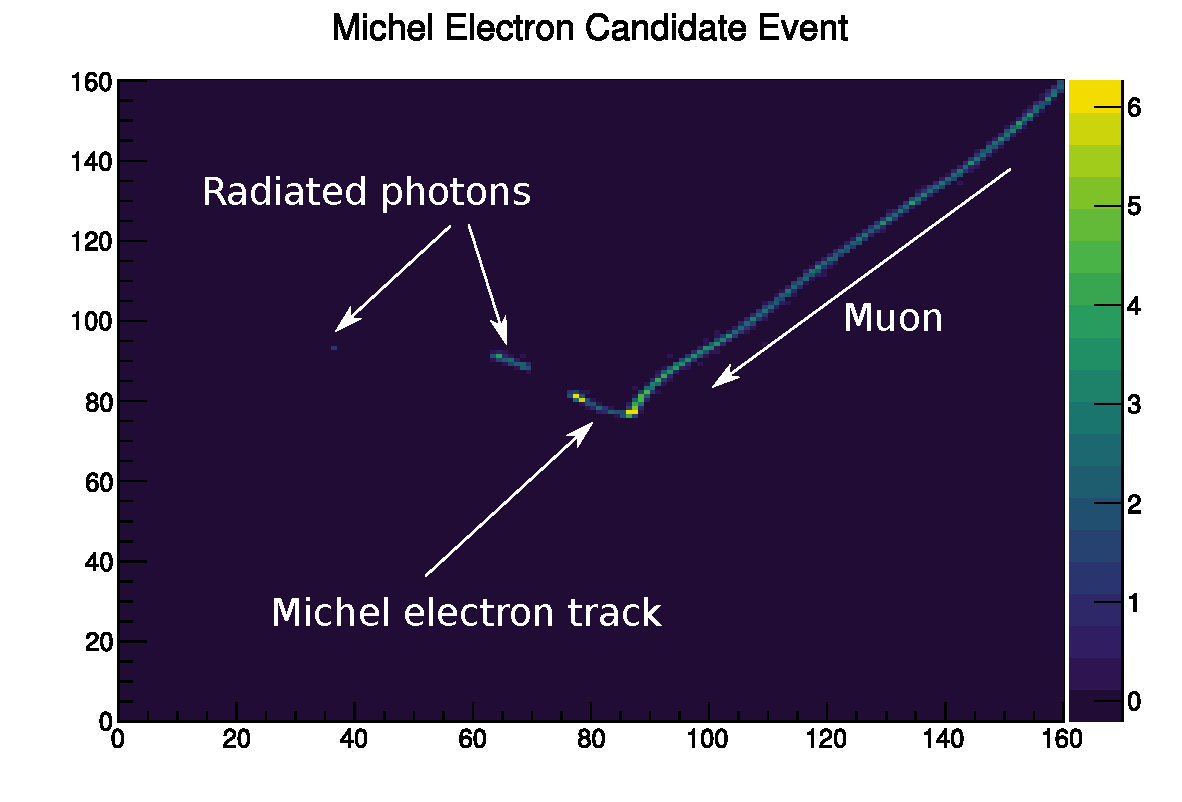
\includegraphics[width=0.7\textwidth]{figures/michel_candidate.pdf}
	\caption[Michel electron candidate event from ProtoDUNE--SP data.]{Michel 
	electron candidate event from ProtoDUNE--SP data.}
	\label{fig:michel_event}
\end{figure}

\section{Michel Electrons in Liquid Argon}
\section{Electromagnetic Energy Loss in Liquid Argon at 0--60 MeV}
\section{Michel Electron Event Selection}
\section{Michel Electron Energy Reconstruction}
\section{Reconstructed Michel Electron Spectrum}
